It's worth noting that in the discussion on the probability of tunneling it is more likely the higher the energy, but the cross section for fusion becomes smaller, so it's a tradeoff. Specifically for the pp-chain the numbers are
\begin{align}
	Z_A=Z_B=1 && \mu = \frac{1}{2}m_p && \mu c^2 = \SI{0.94}{\giga\electronvolt}
\end{align}
giving us 
\begin{equation}
	E_G \approx \SI{500}{\kilo\electronvolt}
\end{equation}
therefore the probability of tunneling is
\begin{equation}
	P=e^{-\sqrt{500}} = \SI{2e-10}{}
\end{equation}
Let's check what this means for the sun. The number of particles in the sun's core is
\begin{equation}
	N = 0.1 \frac{M_\mathSun}{m_p} \sim \SI{e48}{}
\end{equation}
So even though the probability of tunneling is low, it definitely happens. To find the rate of the interactions we insert this into~\ref{fusionrate}:
\begin{align}
	r_{xi} &= \int\sigma n \diff{n}{v}\dd v\\
	&= \int \sigma \sqrt{\frac{2E}{\mu}}\diff{n}{E} \dd E\\
\end{align}
where
\begin{align}
	\diff{n}{E} &= n_i\frac{2}{\sqrt{\pi}}\frac{\sqrt{E}}{\ins{k_B T}^{3/2}}e^{-\frac{E}{k_B T}}\\
	\sigma &= \frac{S}{E}e^{-\sqrt{E_G/E}}\\
	S &= \frac{\pi \hbar^2}{2\mu}
\end{align}
giving us
\begin{align}\label{rate_int}
	r_{xi} &= n_i n_x\ins{\frac{1}{k_B T}}^{3/2}\sqrt{\frac{8}{\pi\mu}}\int e^{-\ins{E/K_B T+\sqrt{E_G/E}}} \dd E
\end{align}
to figure out which particles are most responsible for the fusion process, the high energy ones or the low energy ones, if we designate
\begin{equation}
	f(x) = e^{-\ins{E/K_B T+\sqrt{E_G/E}}} 
\end{equation}
then it looks like
\begin{figure}[!htb]
	\centering
	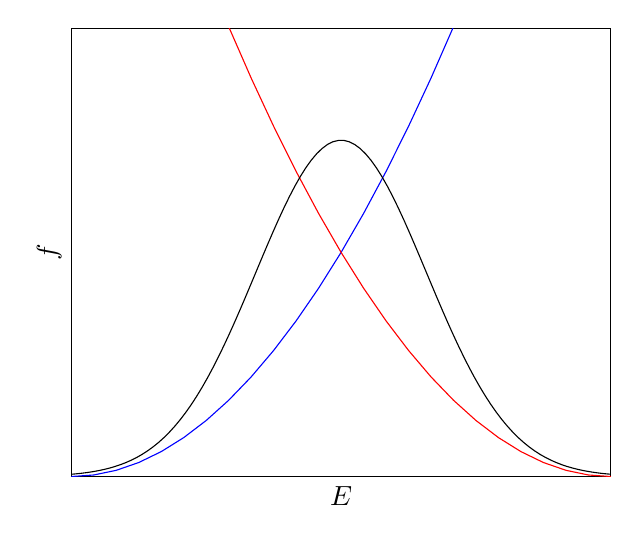
\begin{tikzpicture}
		\begin{axis}[xlabel=$E$, ylabel=$f$, ymin=0, ymax=2, xmin=0, xmax=2, ticks=none]
			\addplot[domain=0:2, color=blue]{x^2};
			\addplot[domain=0:2, color=red]{(2-x)^2};
			\addplot[domain=0:2, color=black, samples=100]{1.5*e^(-5*((x-1)^2))};
		\end{axis}
	\end{tikzpicture}
	\caption{The portion of mass of the universe by element in the universe's early times.}
\end{figure}
and the peak is found at
\begin{equation}
	E_0 = \ins{\frac{k_B T}{2}}^{2/3}E_G^{1/3}
\end{equation}
and specifically for the Sun
\begin{equation}
	E_0 = \SI{5}{\kilo\electronvolt}
\end{equation}
Next we want to solve~\ref{rate_int}. It's not analytically solvable so we approximate it. What's often done in astrophysics is that we approximate things to a power law. Our function looks like this:
\begin{equation}
	r_{xi} = An^2f(T)
\end{equation}
a power law approximation for this would look like
\begin{equation}
	r_{xi} \approx An^2T^\beta
\end{equation}
\begin{wrapfigure}[24]{r}{0pt}
	\begin{tikzpicture}
		\begin{axis}[xlabel=$\log(T)$, ylabel=$\log(r)$, ymin=0, ymax=2, xmin=0, xmax=2, ticks=none]
			\addplot[domain=0:2, color=blue]{x^(1/2)};
			\addplot[domain=0:2, color=red]{x/2+0.5};
		\end{axis}
	\end{tikzpicture}
	\caption{The portion of mass of the universe by element in the universe's early times.}
\end{wrapfigure}
Why do we do this? Often in astrophysics we look at relationships between values of parameters which span very large ranges, often entire orders of magnitude.\ for this reason instead of plotting regular linear graphs, we use log-log graphs. If we take a taylor series at some point and look at the first order it's a linear function. A linear line on a log-log graph fits a function of the form \(T^\beta \). Back to the case of our Sun
\begin{align}
	r_{xi} = An_i n_x f(T) = A\rho_i\rho_x T^\beta
\end{align}
and if we define
\begin{align}
	x_i = \frac{\rho_i}{\rho} && x_x = \frac{\rho_x}{\rho}
\end{align}
then
\begin{equation}
	r_{xi} = r_0x_i x_x\ins{\frac{\rho}{\rho_0}}^2\ins{\frac{T}{T_0}}^\beta
\end{equation}
where \(r_0,\rho_o,T_0\) are parameters we find from the fit. The amount of energy produced from all the fusion is
\begin{equation}
	\dd E = E_0 r_{xi}\dd t \dd V
\end{equation}
and inserting what we found so far
\begin{equation}
	\dd E = E_0r_0x_i x_x\ins{\frac{\rho}{\rho_0}}^2\ins{\frac{T}{T_0}}^\beta \dd V \dd t
\end{equation}
which we are able to rewrite to an integral over the mass by using \(\dd m = \rho\dd V\):
\begin{equation}
	\dd E = \ins{\frac{E_0r_0}{\rho_0}}x_i x_x\ins{\frac{\rho}{\rho_0}}\ins{\frac{T}{T_0}}^\beta \dd m \dd t
\end{equation}
where we can define
\begin{equation}
	\epsilon_0 = \frac{E_0r_0}{\rho_0}
\end{equation}
which has units of energy produced per gram material per second, giving us
\begin{equation}
	\diff[2]{E}{m}{t} = \epsilon_0x_i x_x\frac{\rho}{\rho_0}\ins{\frac{T}{T_0}}^\beta
\end{equation}
and if we insert \(\beta=4\) which fits our Sun and
\begin{align}
	\epsilon_0 = \SI{0.1}{\erg\per\gram\per\second} && \rho_0 = \SI{}{\gram\per\centi\meter^3} && T_0 = \SI{e7}{\kelvin} && x_i=x_x=0.7
\end{align}
then we find
\begin{equation}
	\epsilon_\mathSun = \SI{7.4}{\erg\per\gram\per\second}
\end{equation}
then the luminosity produced is
\begin{align}
	\dd L = \epsilon\dd m = \epsilon\cdot 4\pi r^2\dd r\rho
\end{align}
which gives us
\begin{equation}
	\diff{L}{r} = \epsilon\cdot4\pi r^2 \rho
\end{equation}
\subsection{Diffusion of Photons}
\begin{figure}[!htb]
	\centering
	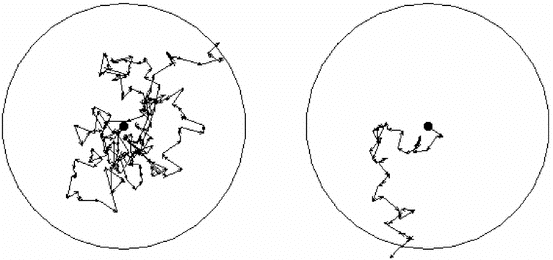
\includegraphics[width=0.75\textwidth]{images/Example-of-Compton-scattering-Brownian-motion-Random-walk-of-a-photon.png}
	\caption{Example of Compton scattering Brownian motion (Random walk) of a photon.}
\end{figure}
Suppose we have a star and inside a photon is created in the middle and moves around inside until it reaches the outside. This process is called a random walk. Each step is of length \(\lambda \) and the star's radius is \(R\). 
\begin{align}
	R^2 &= \left\lvert\vec R \right\rvert^2 = \left\lvert\sum \vec r_i \right\rvert^2\\
	&= \sum\limits_i\sum\limits_j \vec r_i\cdot\vec r_j\\
	&= \sum\limits_{i=1}^N \lvert r_i \rvert ^2 + \sum\limits_{i\neq j}\vec r_i\cdot\vec r_j\\
	&= N\lambda^2
\end{align}
therefore the number of steps until the photon escapes is
\begin{equation}
	N = \ins{\frac{R}{\lambda}}^2
\end{equation}
some typical numbers are
\begin{align}
	R = R_\mathSun && \lambda \approx \SI{0.1}{\centi\meter}
\end{align}
which gives us
\begin{equation}
	N \approx \SI{5e23}{}
\end{equation}
if we want the distance the photon will travel in total then
\begin{align}
	d = \lambda\cdot N \approx \SI{4e22}{\centi\meter} = \SI{16}{\kilo\parsec}
\end{align}
and the time it takes the photon to travel this distance is
\begin{equation}
	t = d/c \approx \SI{50000}{\year}
\end{equation}
If want a more accurate description of the process, we can use the diffusion equation. We won't develop it from scratch but begin from Fick's Diffusion Law (A development from scratch can be found in Feynman's lectures volume 1 chapter 42):
\begin{equation}
	\vec J = -D \nabla n
\end{equation}
where \(J\) is the flux of particles, \(D=\frac{\lambda v}{3}\) is the diffusion parameter. We'll use this formula for photons. The free traversal is given by \(\lambda = \frac{1}{\sigma n} = \frac{1}{\kappa\rho}\) where \(\sigma \) is the action cross section and \(\kappa = \frac{\sigma}{\overline{m}}\) is the opacity. So for photons we'll perform the substitutions
\begin{align}
	v \rightarrow c && D \rightarrow \frac{\lambda c}{3} = \frac{c}{3\kappa\rho} && \rho \rightarrow u_{rad} = aT^4 && J \rightarrow f_{rad} = \frac{L_r}{4\pi r^2}
\end{align}
which gives us
\begin{equation}
	\frac{L_r}{4\pi r^2} = f_{rad} = -\frac{1}{3}\frac{c}{\kappa\rho}\diff*{aT^4}{r}
\end{equation}
rearranging differentiating we find
\begin{equation}
	\diff{T}{r} = -\frac{3}{4ac}\frac{\kappa\rho}{T^3}\frac{L_r}{4\pi r^2}
\end{equation}
In conclusion we have four differential equations:
\begin{align}
	\diff{P}{r} = -G\frac{M_r\rho}{r^2} && \diff{M_r}{r} = 4\pi r^2\rho \\
	\diff{L_r}{r} = 4\pi r^2\rho\epsilon && \diff{T}{r} = -\frac{3}{4ac}\frac{\kappa\rho}{T^3}\frac{L_r}{4\pi r^2}
\end{align}
together with the state equation \(P\), the energy production equation \(\epsilon \), and the opacity \(\kappa \) we have all the tools we need to describe the structure of stars.